\chapter{Introduction}

\section{Contexte de la recherche}

La surpopulation est l’un des principaux maux de ce XXI\textsuperscript{e} siècle, auquel l’humanité doit faire face. En effet, selon un rapport des Nations Unies, la population mondiale serait de 7,3 milliards aujourd’hui, alors que 5,3 milliards d’êtres humains seulement étaient recensés en 1990. De plus, les projections réalisées pour les prochaines décennies ne s’annoncent pas encourageantes ; à savoir 8,5 milliards pour 2030, 9,7 milliards pour 2050 et 11,2 milliards pour 2100 \citep{UnitedNations2017}. Les causes de cette inflation d’envergure sont diverses et varient selon les continents. Par exemple, les pays en développement sont ceux qui montrent les plus forts taux de fertilité, tandis que les pays développés font, quant à eux, face à un certain vieillissement de leur population. Aussi, l’espérance de vie de la population mondiale s’est accrue de manière significative, et ce, principalement en raison des avancées médicales ainsi que de l’augmentation de la production agricole. En effet, les Nations Unies recensent 901 millions de personnes dont l’âge est supérieur à 60 ans. De plus, les prévisions pour les prochaines décennies annoncent 1,4 milliard d’individus en 2030 et 2,1 milliards en 2050 \citep{UnitedNations2015a}.

Dans un premier temps, le vieillissement que connaît la population, majoritairement celle des pays développés, entraîne nécessairement un plus grand nombre de personnes dont l’autonomie se retrouve fortement diminuée, voire complètement perdue. Ce déclin d’autonomie peut être corrélé aux maladies neurodégénératives (\textit{p. ex.} la maladie d’Alzheimer, la maladie de Parkinson, la maladie de Huntington, \textit{etc.}), mais également aux différents handicaps (handicap physique, sensoriel ou intellectuel). Selon la gravité de la perte d’autonomie engendrée par ces pathologies, une assistance rigoureuse demeure nécessaire, car les personnes touchées requièrent une prise en charge relativement constante \citep{Association2017}. Actuellement, les acteurs de la prise en charge des malades sont majoritairement leurs proches \citep{Paraponaris2012}. Néanmoins, ceux-ci doivent alors assumer les conséquences aussi bien sur le plan personnel et émotionnel qu’au niveau social et financier \citep{Association2017}.

Dans un second temps, la forte croissance observée depuis les années 1990 jusqu’à nos jours entraîne un exode rural important. D’après un autre rapport produit par \cite{UnitedNations2017a}, la proportion de résidents urbains devrait atteindre 61\% de la population mondiale dans les prochaines années. Ainsi, de plus en plus de mégapoles se créent (seulement 4 villes affichaient ce statut en 1975, pour 36 aujourd’hui), et tendent à devenir de plus en plus grosses \citep{UnitedNations2017a}. En effet, d’ici à 2025 l’Asie pourrait compter, à elle seule, pas moins de 10 villes dont la population serait supérieure à 40 millions d’habitants. De plus, cette croissance démographique mènera à une dégradation globale de l’environnement et des changements climatiques importants, car il faudra produire de plus en plus de ressources vitales, ce qui provoquera indubitablement un afflux toujours plus conséquent de pollution. De la même façon, le coût global de la vie (logements, nourriture, santé, \textit{etc.}) augmentera, à terme, de façon manifeste \citep{UnitedNations2017a}.

Les récents progrès en matière de technologies de l’information et de microélectronique ont permis de faire émerger de nouveaux concepts comme celui de l’ \ac{IAm}. Ce concept peut être traduit par une couche d’abstraction où l’informatique se retrouve au service de la communication entre les objets et les personnes. En pratique, il s’agit d’enrichir l’environnement dans lequel l’Homme évolue avec la technologie afin d’en extraire le contexte et apprendre son comportement pour prendre des décisions et lui porter assistance \citep{Sadri2011}. L’Intelligence Ambiante se retrouve notamment dans les habitats intelligents, à l’intérieur desquels, différents types de capteurs et d’effecteurs statiques et portables sont utilisés afin de récolter des données. Parmi ceux-ci, il est possible de retrouver des antennes RFID, des capteurs infrarouges et ultrasons, des contacteurs magnétiques et des accéléromètres. La production de telles données permet alors d’apporter de l’assistance et du confort au résident, mais également d’évaluer sa santé mentale et physique \citep{Rashidi2013, Haux2016, Harris2016, Johnson2018}.

Pour l’instant et dans une optique de court terme, les habitats intelligents demeurent d’excellents vecteurs d’assistance pour les personnes touchées par une perte d’autonomie partielle ou totale. De plus, s'ils permettent de compenser les lourdes dépenses que représentent leur prise en charge pour les systèmes de santé. Ils peuvent également à soulager les proches aidant vis-à-vis de la quantité de stress qu’ils éprouvent. À titre d'exemple, le rapport publié par \cite{Prince2016} rapporte que 47 millions de personnes sont actuellement affectées par un trouble neurocognitif ce qui, selon une estimation, coûterait 818 milliards de dollars US à l'échelle mondiale. Néanmoins, les habitats intelligents pourraient tendre à devenir de plus en plus indispensables à long terme. En effet, ceux-ci pourraient avoir un rôle important dans les innovations d’urbanisme à venir, afin d’atténuer les effets engendrés par la surpopulation. Selon un rapport d’UN-Habitat, l’urbanisation représenterait le meilleur compromis face à l’augmentation croissante de la population, car l’activité humaine se retrouverait alors concentrée dans des surfaces limitées, ce qui réduirait l’ampleur des dommages environnementaux \citep{UNFPA2007}. Cependant, cela ne sera possible que si l’urbanisme actuel subit des améliorations significatives, où l’objectif est la conception de villes plus compactes, intégrées socialement, connectées, qui favorisent le développement urbain et qui sont résistantes aux changements climatiques \citep{UNFPA2007}.

Ce projet de thèse ne traitera, cependant, que de la problématique générale de l'assistance aux personnes en perte d'autonomie. Ainsi, les sections suivantes ont pour objectif de définir les notions clés inhérentes à celle-ci.

\section{L'activité humaine}

La notion d'activité humaine dans la problématique de l'assistance aux personnes affectées par une perte d'autonomie demeure fondamentale. C'est pourquoi il convient de la définir de façon appropriée. Dans le domaine de la santé, il est convenu que l'utilisation du terme activité fait directement référence au concept d'activité de la vie quotidienne (\acl{ADL} ou \acs{ADL}) introduit et présenté par \cite{Katz1963}. Il regroupe un ensemble d'activités permettant de mesurer l'habileté pour un individu à maintenir sa santé et son autonomie (\textit{p. ex.} préparer à manger, s'habiller, se laver, \textit{etc.}). Ainsi, le succès ou l'échec dans la réalisation de ces tâches constitue, pour les professionnels de la santé, une mesure fiable pour quantifier la perte d'autonomie d'un patient présentant un handicap dont celle-ci en est soit une cause, soit une conséquence. Ceci permet alors d'adapter le type et le niveau d'assistance approprié pour chacun d'entre eux \citep{Giovannetti2002}. Depuis les travaux de \cite{Katz1963}, les chercheurs \cite{Lawton1969} ont proposé un regroupement des \acs{ADL}s en deux ensembles distincts qui sont :

{\textbf{Les activité basiques (\acl{BADL} ou \acs{BADL})} regroupent l'ensemble de toutes les activités fondamentales aux besoins primaires d'une personne. Par exemple, se déplacer sans aucun outil d'assistance (béquille, canne, \textit{etc.}), se laver, se nourrir, se coucher, se lever, \textit{etc.} Ces activités sont généralement composées de très peu d'étapes et ne requièrent aucune planification pour être accomplies avec succès.

{\textbf{Les activités instrumentalisées (\acl{IADL} ou \acs{IADL})} sont, quant à elles, l'ensemble des activités qui nécessitent une certaine planification et qui permettent de statuer sur l'autonomie d'une personne en société. On y retrouve, par exemple, l'appel téléphonique, la préparation d'un repas ou encore la gestion de l'argent. Aussi, ces activités requièrent souvent beaucoup plus d'étapes dans leur exécution que les \acsp{BADL}.

Finalement, ce regroupement a été étendu par \cite{Rogers1998} afin d'y inclure un troisième et dernier ensemble d'activités laissées pour compte jusqu'alors. Il s'agit des \ac{EADL} qui comprend toutes les activités qui nécessitent une certaine adaptation ou un apprentissage pour être menées à bien. Par exemple, utiliser un nouvel appareil électronique dans la maison représente une activité nécessitant un apprentissage et une certaine adaptation pour l'habitant.

Maintenant que la notion fondamentale d'activité a été définie, il est nécessaire d'expliquer en quoi elle est au c\oe{}ur du fonctionnement même des habitats intelligents puisque l'objectif de ceux-ci est d'offrir à leurs résidents une assistance adaptée grâce à la reconnaissance de leurs activités.

\section{La reconnaissance d'activités}

La reconnaissance d'activités est un domaine qui fait partie de l'Intelligence Artificielle (\acs{IA}). De nos jours, ce dernier suscite un intérêt toujours plus grandissant chez les chercheurs pourtant, sa première définition n'est pas récente. En effet, selon \cite{Schmidt1978}, la reconnaissance d'activités peut se traduire comme la découverte du but qu'un acteur souhaite atteindre à partir d'une séquence d'actions qu'il est en train de réaliser. Ainsi, la reconnaissance d'activités est la déduction d'une suite d'actions dans l'espace et le temps (la structure d'activité) déterminée et exécutée par une entité qu'un observateur va alors chercher à reconnaître.

Depuis, \cite{Roy2013} ont proposé de caractériser la reconnaissance d'activités par la relation qu'il existe entre l'observateur (\textit{p. ex.} l'habitat intelligent) et l'observé (\textit{p. ex.} le résident). Ainsi, il demeure possible de mettre en place un découpage de la reconnaissance d'activités en différents types, selon le comportement que l'observé adopte envers l'observateur. Trois comportements distincts ont donc été recensés : positif, négatif ou neutre. Dans le premier cas, l'observé va agir de sorte à faciliter et même collaborer avec l'observateur dans son processus de reconnaissance. Pour ce faire, l'observé peut, par exemple, poser des questions à l'observateur en cas de doutes. Cependant, appliquer un tel type de reconnaissance relève de l'impossible lorsque les résidents des habitats intelligents sont affectés par des troubles cognitifs comme la maladie d'Alzheimer. En effet, la nécessité d'adapter son comportement pour assister l'observateur dans son processus requiert une forte augmentation de la charge cognitive de l'habitant, ce à quoi, il leur est pratiquement impossible de faire face. Dans le second cas, où l'observé adopte un comportement négatif envers l'observateur, il va essayer délibérément, et par tous les moyens, d'empêcher le bon déroulement de la reconnaissance. Néanmoins, ceci n'arrive jamais avec les résidents atteints de l'Alzheimer, mais pourrait parfaitement se produire dans le cas d'autres maladies et/ou handicaps. Les personnes atteintes d'Alzheimer entrent plutôt dans la dernière catégorie de comportement, où l'observé n'agit ni pour aider ni pour empêcher le processus de reconnaissance.

La présentation de ces trois types de reconnaissance vient clore la définition générale de la reconnaissance d'activités. Il est maintenant nécessaire de s'intéresser à l'intégration de cette problématique au sein des environnements intelligents.

\section{La reconnaissance d'activités dans les environnements intelligents}

Depuis sa définition initiale, de nombreux travaux ont fait évoluer la reconnaissance d'activités afin que celle-ci puisse s'adapter au contexte bien spécifique des environnements intelligents \citep{Patterson2005, Boger2006, Bouchard2007, Ghayvat2018}. L'objectif majeur de ces adaptations était de remanier le concept d'environnement ambiant, afin qu'il puisse s'unir avec la problématique de la reconnaissance d'activités.

De ce fait, la première extension à la définition de ce processus appliquée de manière concrète à ces environnements a été décrite par \cite{Patterson2005}. Leur recherche indique que les observations doivent être réalisées à partir des données fournies par des capteurs de bas niveau. Cette nouvelle vision vient directement s'inscrire dans l'ère de l'informatique ubiquitaire \citep{Weiser1991} et devient, par conséquent, beaucoup plus pertinente face à la réalité du problème. L'observé évolue alors dans un environnement composé de différents capteurs, dont le rôle est de récolter les variations qui sont produites par les interactions entre l'acteur et son environnement. Par conséquent, ce sont ces changements qui vont permettre à l'observateur de réaliser le processus de reconnaissance d'activités.

Plus récemment, en se basant sur les travaux précédents de \cite{Patterson2005}, \cite{Roy2013} ont proposé une liste de quatre problématiques pour accomplir le processus de reconnaissance d'activité au sein des environnements intelligents. La première concerne la récolte des valeurs d'un ensemble hétérogène de capteurs de manière uniforme. En d'autres termes, il s'agit d'offrir la possibilité de recueillir toutes les données produites par l'ensemble de capteurs au travers d'une interface unique, où cette dernière fait totalement abstraction du protocole de communication pour chaque capteur (\textit{p. ex.} RFID, Bluetooth, Wi-Fi, I\textsuperscript{2}C, \textit{etc.}). Le second défi identifié par \cite{Roy2013} est l'interprétation de ces valeurs pour en déduire de l'information intelligible, comme la localisation du résident au sein de l'environnement. Ensuite, la troisième problématique est d'être en mesure de déterminer les actions qui sont effectuées par l'habitant \textit{via} l'interprétation des valeurs renvoyées par les capteurs. Enfin, le dernier défi mentionné par les auteurs concerne l'interprétation de la suite d’actions produites en une activité de plus haut niveau.

Pour répondre à ces quatre problématiques, \cite{Roy2013} ont proposé un modèle de reconnaissance d'activités multicouche dont la représentation graphique est donnée en figure \ref{fig:activity_recognition}. Les quatre couches qui composent ce modèle sont indépendantes les unes des autres. Chaque couche a pour objectif de ne répondre qu'à une seule problématique en particulier et doit fournir à la couche supérieure le résultat du traitement achevé. Ainsi, chacune des problématiques peut être traitée séparément.

\begin{figure}[H]
	\centering
	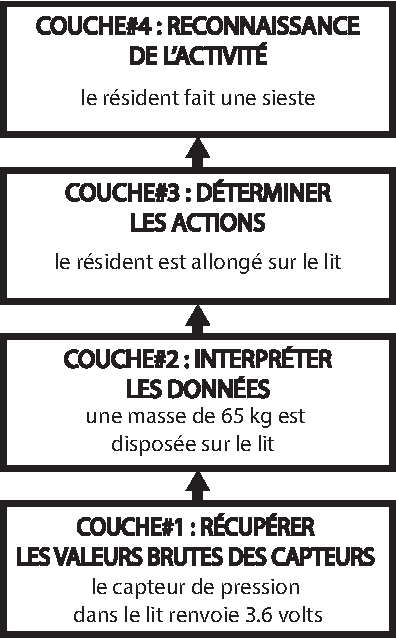
\includegraphics[width=6cm]{activity_recognition.pdf}
	\caption{Représentation multicouches de la reconnaissance d'activités dans les environnements intelligents.}
	\label{fig:activity_recognition}
\end{figure}

En définitive, il est donc possible d'effectuer une reconnaissance d'activités au sein d'un environnement intelligent à partir de capteurs de bas niveau\textemdash à condition que les différentes problématiques énoncées précédemment soient respectées tout au long du processus.

\section{Les habitats intelligents et les \textit{wearable devices}}

Au cours des dix dernières années, de nombreux travaux concernant les environnements intelligents et plus particulièrement, les habitats intelligents ont vu le jour. Pour reconnaître les activités des résidents, ceux-ci ont adopté des architectures sensiblement identiques, où les valeurs des capteurs sont centralisées en une entité unique (un serveur) qui va, à elle seule, exécuter toutes les couches de la reconnaissance d’activités \citep{Bouchard2014, Hu2016}. Néanmoins, certaines distinctions demeurent entre ces différentes implémentations. Par exemple, le \ac{LIARA} \citep{Bouchard2014} et le Laboratoire de \ac{DOMUS} \citep{Giroux2009} représentent les habitats intelligents hérités du monde de l’industrie. Les autres implémentations d'habitats intelligents comme Gator-Tech \citep{Helal2005}, MavHome \citep{DJCook2003}, CASAS \citep{Cook2013} ou encore Amiqual4home \citep{Lago2017} reposent toutes, quant à elles, sur des architectures par composants. Cependant, ces habitats intelligents connaissent certaines limitations. En effet, bien que les architectures centralisées simplifient l'utilisation des algorithmes de reconnaissance d'activités, elles ont un impact significatif sur la fiabilité de fonctionnement du système de reconnaissance et donc sur la sécurité du résident qui occupe l'habitat. Bien que de nouveaux travaux essayent de répondre à cette problématique \citep{Cook2013, Plantevin2018}, les habitats intelligents restent également, encore très dispendieux.

Par ailleurs, les recherches réalisées dans la reconnaissance d'activités au sein d'un habitat intelligent se sont intéressées, en grande partie, à reconnaître les activités d'un unique habitant dans l'environnement (mono-résident) \cite{VikramadityaJakkula2007, VanKasteren2008, Inomata2009, Ghazvininejad2011, Belley2014, Fortin-Simard2015}. Bien que très performantes, ces solutions se sont retrouvées défaillantes lorsque l'habitat est occupé par plusieurs résidents (multi-résident). Ce cas de figure constitue pourtant une problématique bien plus proche de la réalité actuelle des habitats intelligents. De nouvelles techniques de reconnaissance d'activités ont donc été proposées \citep{Crandall2009, Cook2009, Alemdar2013, Ayuningtyas2014, Emi2015, Mokhtari2018}. Plusieurs d'entre elles \citep{Mihailidis2004, Tunca2014} se sont alors tournées vers l'utilisation de \textit{wearable devices}, beaucoup plus accessibles financièrement. D'autre part, grâce à la miniaturisation de ces appareils, ceux-ci tendent à être de moins en moins considérés comme intrusifs par leur utilisateurs \citep{Gaskin2017}. En plus de la reconnaissance d'activités mono-résident et multi-résidents, ces capteurs portables ont permis l'ouverture de nouveaux horizons de recherche et sont principalement utilisés pour la surveillance de la santé, la réhabilitation physique, la détection de chutes, \textit{etc.} \citep{Patel2012, Mukhopadhyay2014, Delahoz2014}.

L'augmentation de l'utilisation des \textit{wearable devices} au sein des habitats intelligents a fait émerger de nouvelles problématiques. Dans un premier temps, puisque ceux-ci se trouvent placés sur les résidents, il devient alors possible d'envisager de nouveaux types de reconnaissance permettant d'améliorer la qualité de l'assistance proposée. Néanmoins, puisque les différentes architectures recensées dans la littérature n'ont pas été initialement prévues pour accueillir ce type de matériel, les \textit{wearable devices} se retrouvent très mal, voir nullement intégrés à celles-ci. Il apparaît donc primordial de s'intéresser à une manière de mieux les intégrer, dans le but de proposer un processus de reconnaissance combinée entre les données fournies, à la fois par les capteurs ambiants et portables, ce qui apparaît difficilement faisable actuellement tant en termes d'intégration matérielle que d'exploitation logicielle. En effet, les dispositifs actuels exploitent uniquement les données qu'ils génèrent eux-mêmes, mais il apparaît crucial de proposer une solution afin de pouvoir utiliser, de manière générique, les données générées par plusieurs \textit{wearable devices}.

\section{Définition du projet de recherche}
\label{sec:def_proj}

\textbf{\hl{Retravailler cette section}}

Ce projet de thèse s'articule donc autour de l'exploitation des \textit{wearable devices} ainsi que de l'interopérabilité de ces derniers avec l'utilisation de l'intelligence ambiante au sein des habitats intelligents. Plus particulièrement, ce projet de thèse permettra de répondre aux questions suivantes :

\begin{enumerate}
	\item
		\label{question:1}
		Quels nouveaux apports, en matière d'intelligence, les \textit{wearable devices} vont permettre de proposer aux résidents des habitats intelligents afin d'améliorer l'assistance qui leur est requise ?

	\item
		\label{question:2}
		Comment optimiser l'intégration des \textit{wearable devices} afin qu'ils puissent être utilisés en combinaison avec les capteurs statiques présents dans les habitats intelligents pour réaliser une reconnaissance basée sur l'interopérabilité de ces deux méthodes ?

	\item
		\label{question:3}
		Comment valoriser la réutilisation des différents algorithmes employés dans la reconnaissance d'activités avec les \textit{wearable devices} afin de faciliter les expérimentations dans un cadre académique ?
\end{enumerate}

Tout d'abord, différents \textit{wearable devices} permettant de réaliser de nouveaux types de reconnaissances seront développés afin de proposer une meilleure assistance aux résidents de l'habitat intelligents. Ensuite, l'objectif de ce projet de thèse est de mettre en place un framework pour faciliter l'intégration des \textit{wearable devices} au sein des ces environnements. Celui-ci fournira une couche d'abstraction autant envers l'architecture de l'habitat dans lequel il est déployé qu'envers le dispositif lui-même. Enfin, cet outil aura également pour fonction de faciliter l'utilisation de ces appareils, dans un cadre académique, en offrant la possibilité de valider plus rapidement le fonctionnement des prototypes.

\section{Organisation du document}

\textbf{\hl{Retravailler cette section}}

La suite de ce projet de thèse se découpe en trois chapitres. Le \autoref{chap:2} présente, dans un premier temps, les différentes architectures d'habitats intelligents existantes. Dans un second temps, ce chapitre explique plus en détail le processus de reconnaissance d'activité et plus spécifiquement, les différents algorithmes qui sont utilisés pour l'apprentissage et la classification. Ensuite, le \autoref{chap:3} explicite le fonctionnement des \textit{wearable devices} ainsi que les différentes applications de ceux-ci au sein des habitats intelligents.